\documentclass[12pt,oneside]{book}

\title{Application for Promotion to Candidacy}
\author{File Preparation Committee}
\date{2023}

\usepackage[T1]{fontenc}
\usepackage{fourier} % Adobe Utopia

\usepackage[activate={true,nocompatibility},final,tracking=true,kerning=true,spacing=true,factor=1100,stretch=10,shrink=10]{microtype}
\microtypecontext{spacing=nonfrench}

% For better formatting in the table listing referees
\usepackage{array}

% To allow H location for image floating (meaning "right here")
\usepackage{float}

\usepackage[margin=2cm]{geometry}

\setlength{\headheight}{15pt}

% \renewcommand{\thechapter}{\Roman{chapter}}

% Say "A", not "Chapter A", by removing the word \chapter.
\renewcommand{\chaptername}{}

% To include images
% \usepackage{graphicx}

% Tighter lists.
\usepackage{enumitem}
\setlist{noitemsep}

% So I can include other PDFs. Section and page numbering are all handled perfectly.
\usepackage{pdfpages}
% When including slides I do this to make a 2x3 layout:
% \includepdf[pages=-,nup=2x3,delta=5mm 5mm,landscape=false]{filename.pdf}
% \includepdf[pages=-,scale=0.8,pagecommand=\thispagestyle{plain}]{0-0-3-job-description-2011.pdf}

% I was getting errors like this:
% pdfTeX warning: pdflatex (file ./2-4-1-lrts-frbr-book-review.pdf): PDF inclusion: found PDF version <1.7>, but at most version <1.5> allowed
% but this fixes it:
\pdfoptionpdfminorversion=7
% See also
% http://tex.stackexchange.com/questions/11698/pdf-inclusion-found-pdf-version-1-5-but-at-most-version-1-4-allowed

% Suppress warnings like this:
% pdfTeX warning: pdflatex (file ./pdfs/B 2.2.1 Introduction to Data Visualization for Research.pdf): PDF inclusion: multiple pdfs with page group included in a single page
\pdfsuppresswarningpagegroup=1

% For better table formatting
%\usepackage{multirow}
%\usepackage{rotating}
%\usepackage{longtable}

% Put headings in small caps
% http://tex.stackexchange.com/questions/45248/headings-in-uppercase5
% \usepackage{sectsty}
% \allsectionsfont{\mdseries\scshape}
% \sectionfont{\mdseries\scshape}

% Start numbering sections at 0.
\setcounter{section}{-1}
\setcounter{chapter}{-1}

% Nice headers.
\usepackage{fancyhdr}
\pagestyle{fancy}
\fancyhf{}
%  \thepage, \thesubsection etc.  \leftmark is chapter title, \rightmark is section title
% \renewcommand{\headrulewidth}{1pt}
\fancyhead[C]{\nouppercase{\rightmark}} % \leftmark is chapter title, \rightmark is section title
\fancyfoot[L]{Name Here} % \leftmark is chapter title, \rightmark is section title
\fancyfoot[C]{\leftmark} % \leftmark is chapter title, \rightmark is section title % Could use \textcolor{red}{Wong}
\fancyfoot[R]{\thepage} % \leftmark is chapter title, \rightmark is section title

% Found this on Stack Exchange
% TODO Add link
\newcommand{\chaptertitle}{}
\renewcommand{\chaptermark}[1]{\renewcommand{\chaptertitle}{Chapter \thechapter\ #1}}
\renewcommand{\sectionmark}[1]{\markboth{\thesection\ #1}{}}
\renewcommand{\subsectionmark}[1]{\markright{\thesubsection\ #1}}

\renewcommand{\footrule}{\hbox to\headwidth{\color{red}\leaders\hrule height \headrulewidth\hfill}}

\fancypagestyle{plain}{%
  % To make chapter pages look like the other pages.
  % https://tex.stackexchange.com/questions/117328/fancyhdr-does-not-apply-same-header-footer-on-chapter-and-non-chapter-pages
  \fancyhf{}%
  \fancyfoot[L]{Name Here} % \leftmark is chapter title, \rightmark is section title % Could use \textcolor{red}{Wong}
  \fancyfoot[C]{\leftmark} % \leftmark is chapter title, \rightmark is section title % Could use \textcolor{red}{Wong}
  \fancyfoot[R]{\thepage} % \leftmark is chapter title, \rightmark is section title
}

% Turn \url and \href into hyperlinks in PDFs, and pass hyphens option to url package
% (which hyperref calls) to get better line breaks.
% http://tex.stackexchange.com/questions/3033/forcing-linebreaks-in-url?rq=1
\PassOptionsToPackage{hyphens}{url}\usepackage[pdfborder={0 0 0},colorlinks=true,urlcolor=blue]{hyperref}

% With this I can say \link{http://example.com/} and it makes it a hyperlink wrapped in < >
\newcommand{\link}[1]{{\small $<$\url{#1}$>$}}

% Add PDF properties (part of hyperref)
\hypersetup{%
  bookmarksnumbered, % To get A 1.2 etc. into the bookmarks
  pdfauthor={File Preparation Committee},
  pdfsubject={},
  pdftitle={Application for Promotion},
  pdfkeywords={},
  linkcolor=black % Other TOC listings, and internal links, are in red
}

%% Attachments
% \attached puts a short horizontal rule, with some space above and below,
% which I'll follow with a list of the attachments for the section.
% This isn't used, but I'll leave it in just in case.
\newcommand{\attached}{%
\vspace{1em}
\noindent\rule{8cm}{0.4pt}
\newline
\vspace{1em} Attached:
}

%% Candidate's notes
% \candidatenote adds a note from the candidate, formatted (with a
% different typeface) so it looks noticeably different from the rest
% of the file.  The phv font is a Helvetica clone.
\newcommand{\candidatenote}[1] {%
\par\noindent\rule{\textwidth}{1pt}
{\large Candidate's note:}
\begin{quote}
  \fontfamily{phv}\selectfont
  {\small #1}
\end{quote}
}

\begin{document}

\frontmatter

\begin{titlepage}

  \null\vfill

  \begin{center}

    {\Huge
      Application for Promotion
    }
    \vspace{2cm}

    {\Large
      Name Here
    }
    \vspace{1cm}

  {\large
    Position Title

    York University Libraries

    \vspace{1cm}

    dd Month 2023

  }

\end{center}

\vfill
\vfill

{\large
  File Preparation Committee:

  Name One (Associate Librarian) \\
  \indent Name Two (Associate Librarian) \\
  \indent Name Three (Associate Librarian)
}

\hfill

\end{titlepage}

% \begin{abstract}
% ...
% \end{abstract}

% \listoffigures

\tableofcontents

\mainmatter{}

\chapter{Front matter}

\pagenumbering{arabic}

\section{Curriculum vit\ae}

\begin{itemize}
  \item Current CV.\@  The included PDF is shrunk to 95\% of its original size.
\end{itemize}


\includepdf[pages=-,scale=0.95,pagecommand={}]{pdfs/example-2.pdf}

\section{Job description}

\begin{itemize}
  \item Job description (2023)
\end{itemize}


\includepdf[pages=-,scale=0.95,pagecommand={}]{pdfs/example-1.pdf}

\section{Personal statement}

\begin{itemize}
  \item Personal statement from the candidate
\end{itemize}


\includepdf[pages=-,scale=1,pagecommand={}]{pdfs/example-2.pdf}

\renewcommand\thechapter{A}
\chapter{Professional Performance and Knowledge}
% \label{chapter:ppk}

\section{Teaching}

\subsection{Course name}

\begin{itemize}
  \item Included slides (showing that multiple slides can be shown on one page; the arrangement is easily configurable).
\end{itemize}

\candidatenote{
  This is a note from the candidate.  It has a different typeface and stands out from the rest of the file.
}

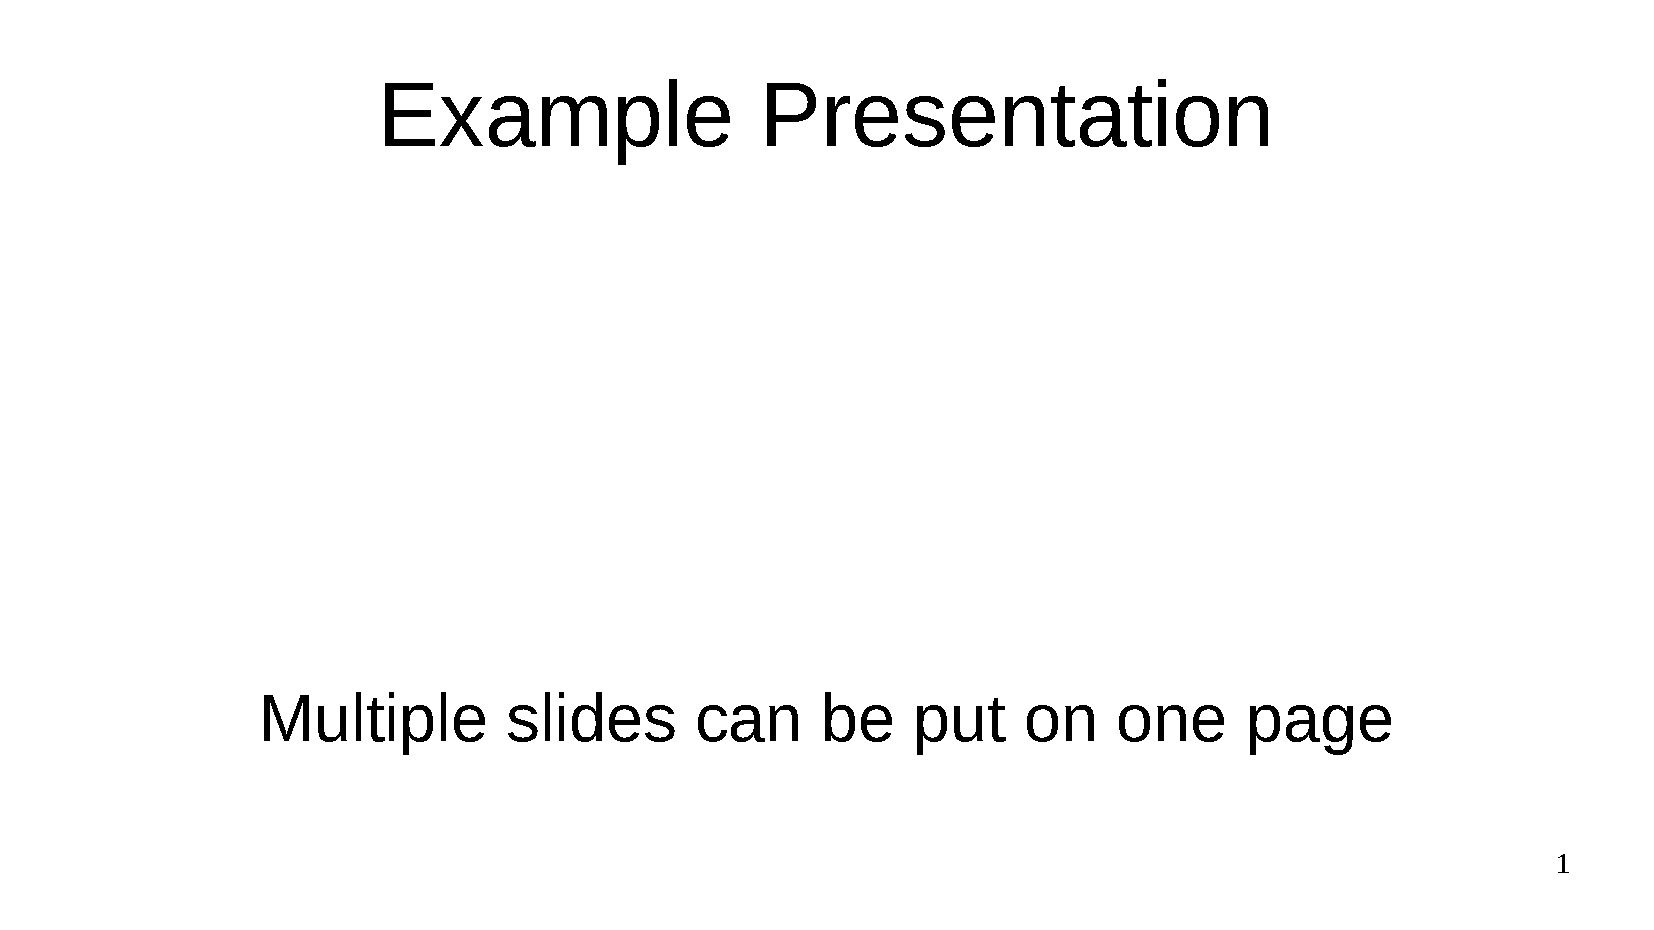
\includepdf[pages=-,nup=1x2,delta=5mm 5mm,landscape=false]{pdfs/example-slides.pdf} % chktex 29

\section{Reference}

\subsection{Example}

\begin{itemize}
  \item Included image.  It is also possible to include images.
\end{itemize}

\begin{figure}[H]
  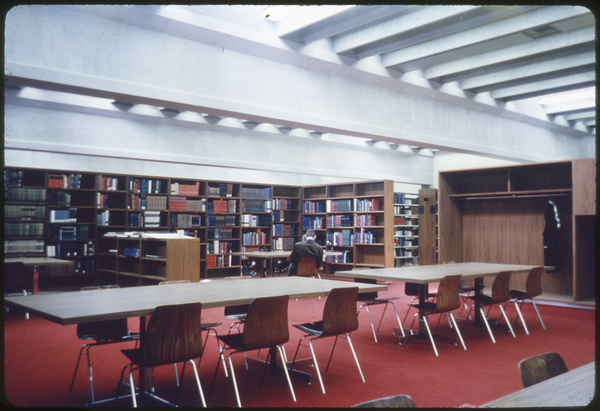
\includegraphics[height=4in]{images/yul 1121686_Medium_sized_JPEG.jpg}
  \caption{The Steacie Science Library in 1965. \\ \href{https://digital.library.yorku.ca/yul-1121686/steacie-science-library-interior-view}{View in YUDL}.}
\end{figure}

\newpage

\renewcommand\thechapter{B}
\chapter{Professional Contributions and Standing}

\section{Publications}

\subsection{``Article Title'' (\textit{Journal Title})}

A citation to the article goes here.  Do not include the article itself.

\vspace{\baselineskip}

[Note: A note from the committee can be added like this, if necessary.]

\newpage

\section{Presentations and Talks}

\subsection{``Title of Talk'' (Conference, 2023)}

\begin{itemize}
  \item Slides from talk.
\end{itemize}

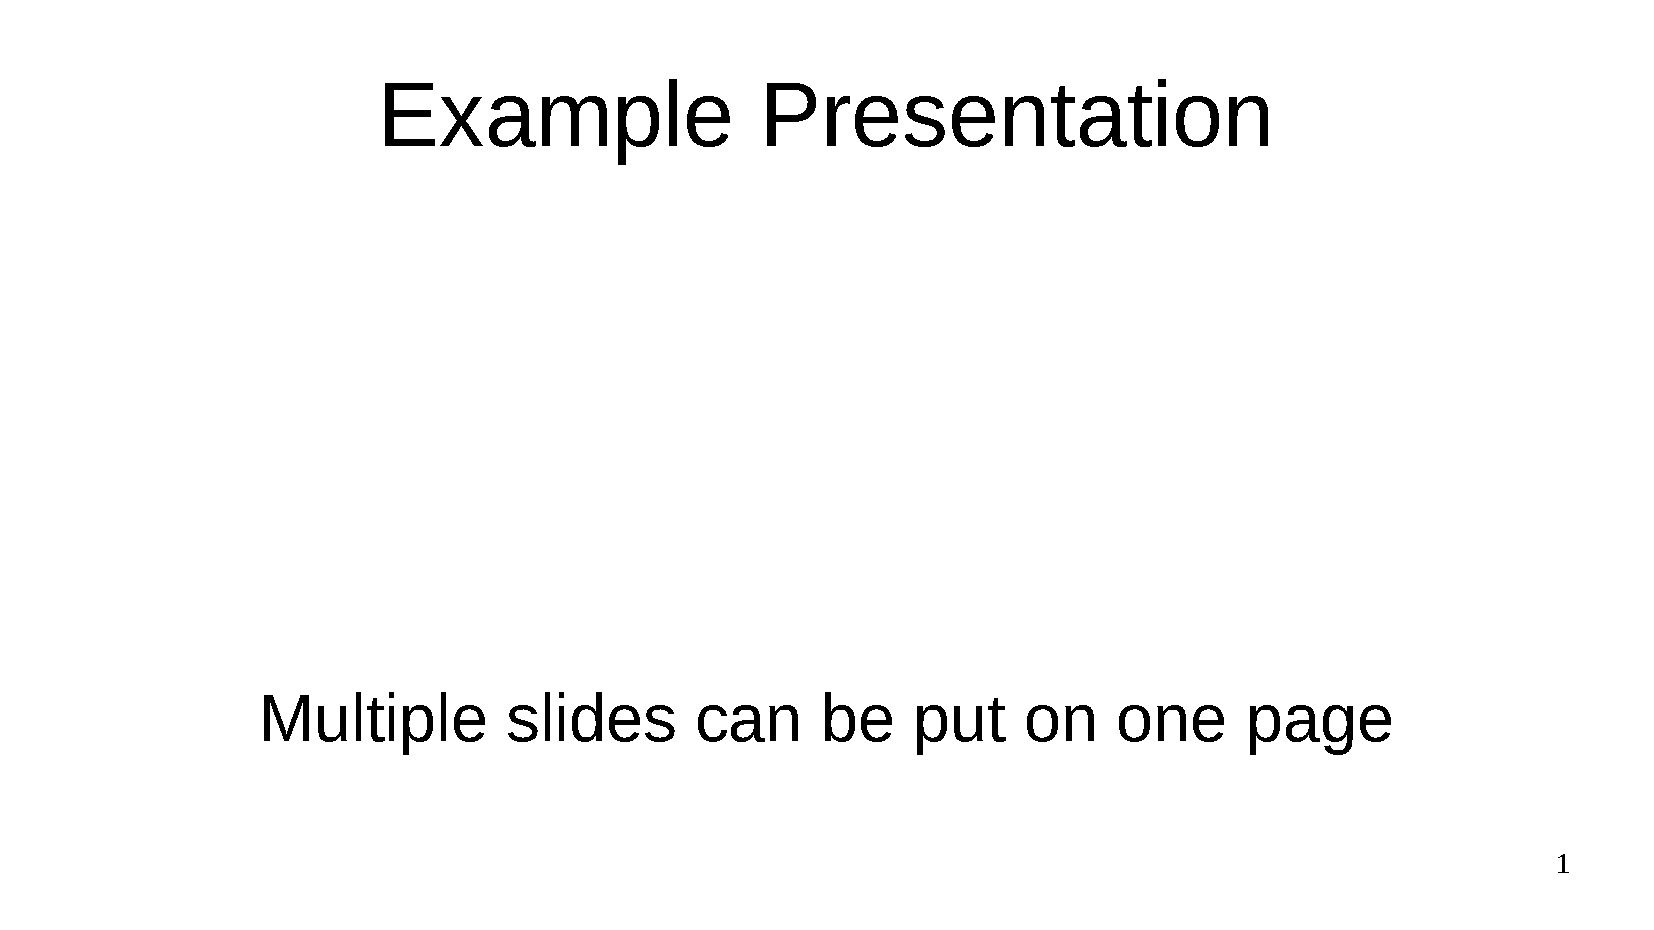
\includepdf[pages=-,nup=2x3,delta=5mm 5mm,landscape=false]{pdfs/example-slides.pdf} % chktex 29

\section{Professional Associations}

\subsection{Association name}

\begin{itemize}
  \item Included PDF described here.
\end{itemize}

\candidatenote{
  This is a note from the candidate.  It has a different typeface and stands out from the rest of the file.
}


\includepdf[pages=-,scale=0.95,pagecommand={}]{pdfs/example-1.pdf}

\renewcommand\thechapter{C}
\chapter{Service}

\section{York University Libraries}

\subsection{A Library Committee}

\begin{itemize}
  \item The annual report of the committee.
\end{itemize}


\includepdf[pages=-,scale=0.95,pagecommand={}]{pdfs/example-1.pdf}

\section{York University}

\subsection{A University Committee}

\begin{itemize}
  \item The annual report of the committee.
\end{itemize}


\includepdf[pages=-,scale=0.95,pagecommand={}]{pdfs/example-1.pdf}

\end{document}
